\section{D. Irga B. Naufal Fakhri}
\subsection{Pemahaman Teori}
\begin{enumerate}
\item CSV

CSV (Comma Separated Values file) adalah sebuah tipe file text biasa yang memiliki penataan khusus yang biasanya berfungsi untuk mengelola data. sesuai dengan namanya file csv memisahkan setiap data menggunakan koma (,).

Format data CSV pertama kali digunakan pada tahun 1978 pada complier FORTRAN 77, kemudian nama CSV baru muncul dan mulai digunakan pada tahun 1983 

Contoh data pada csv:
\lstinputlisting[firstline=0, lastline=2]{src/4/1174066/Teori/1174066.csv}

\item Aplikasi yang bisa menciptakan CSV

Semua aplikasi teks editor seperti notepad++, vscode, sublime ataupun notepad dapat menciptakan CSV termasuk aplikasi spreadsheet seperti Microsoft Excel, Libre Office 

\item Jelaskan bagaimana cara menulis dan membaca file csv di Excel atau spreadsheet

\begin{itemize}
	\item Buka Microsoft Excel 2019-nya lalu buat dokumen baru
	\item Isikan data sesuai dengan kebutuhan, yang paling atas akan menjadi header dari file csv
	\item Setelah memasukkan data, klik file lalu klik Save As
	\item Pilih Browse dan pilih tempat menyimpannya akan dimana
	\item Masukkan nama file pada File Name
	\item Lalu pada Save As Type pilih CSV (comma delimited) (*.csv)
	\item Maka hasil file akan seperti ini
	\lstinputlisting[firstline=0, lastline=2]{src/4/1174066/Teori/1174066.csv}
\end{itemize}

\item Jelaskan sejarah library csv

Module csv mengimplementasikan kelas untuk membaca dan menulis data kedalam format CSV. Hal ini memungkinkan programmer untuk "tulis data ini dalam format yang disukai oleh Excel," atau "baca data dari file yang dihasilkan oleh Excel," tanpa mengetahui detail yang tepat dari format CSV yang digunakan oleh Excel. Pemrogram juga dapat menggambarkan format CSV yang dipahami oleh aplikasi lain atau menentukan format CSV tujuan khusus untuk mereka sendiri.

\item Jelaskan sejarah library pandas

pandas adalah sebuah library open source dan berlisensi BSD yang menyediakan performa yang tinggi, mudah digunakan struktur data dan data analisis untuk python.

\item Jelaskan fungsi-fungsi yang terdapat di library csv
\begin{itemize}
	\item csv.reader
	
	Berfungsi untuk membaca dan mengembalikan data kedalam variable dari file csv.
	Fungsi reader dirancang untuk mengambil data pada setiap baris didalam file dan membuat daftar semua kolom. Kemudian, tinggal dipilih kolom mana yang diinginkan untuk data variabel.
	\lstinputlisting[firstline=9, lastline=22]{src/4/1174066/Teori/1174066_csv.py}
	
	\item csv.writer
	
	Berfungsi untuk menuliskan data dari variable kedalam file csv.
	Fungsi writer akan membuat objek yang cocok untuk menulis. Untuk mengulang data yang ada di atas baris, gunakan fungsi writerow.
	\lstinputlisting[firstline=38, lastline=45]{src/4/1174066/Teori/1174066_csv.py}
	
	\item csv.register\textunderscore dialect
	
	Mendaftarkan dialect pada csv
	\item csv.unregister\textunderscore dialect
	
	Menghapus dialect yang diasosiasi dengan nama dari registry dialect
	
	\item csv.list\textunderscore dialects
	
	Mengembalikan dialect yang diasosiasi dengan nama
	
	\item csv.field\textunderscore size\textunderscore limit
	
	Mengembalikan ukuran field maksimum yang diizinkan oleh parser.
	
	\item csv.DictReader
	
	Berfungsi untuk membaca dan mengembalikan data kedalam variable dictionary dari file csv.
	\lstinputlisting[firstline=24, lastline=36]{src/4/1174066/Teori/1174066_csv.py}
	
\end{itemize}

\item Jelaskan fungsi-fungsi yang terdapat di library pandas
\begin{itemize}
	\item pandas.read\textunderscore csv
	
	Berfungsi untuk membaca dan mengembalikan data kedalam format DataFrame dari file csv.
	\lstinputlisting[firstline=9, lastline=13]{src/4/1174066/Teori/1174066_pandas.py}
	
	\item to\textunderscore dict
	
	Berfungsi untuk membaca dan mengembalikan data kedalam format dictionary dari file csv.
	\lstinputlisting[firstline=15, lastline=19]{src/4/1174066/Teori/1174066_pandas.py}
	
	\item to\textunderscore csv
	
	Berfungsi untuk mengedit data didalam csv dan menulisnya kedalam file csv
	\lstinputlisting[firstline=42, lastline=49]{src/4/1174066/Teori/1174066_pandas.py}
\end{itemize}
\end{enumerate}

%%%%%%%%%%%%%%%%%%%%%%%%%%%%%%%%%%%%%%%%%%%%%%%%%%%%%%%%%%%%%%%%%%%%%%%%%%%%%%%%%%%%%%%%%%%%%%%%%%%%%%%%%%%%%%%%%%%%%%%%%%
\section{Fanny Shafira Damayanti | 1174069}
\subsection{Pemahaman Teori}
\begin{enumerate}
\item Fungsi CSV, sejarah dan contoh

CSV (comma separated value) digunakan pada tahun 1983 merupakan suatu tipe file yang digunakan untuk pengolahan informasi yang dihasilkan spreadsheet yang di proses melalui mesin analitik. CSV juga digunakan sebagai file yang agnostik karena bisa digunakan olej berbagai database untuk backup data.

Contoh :

\lstinputlisting[firstline=7, lastline=28]{src/4/1174069/Teori/1174069_csvteori.py}

\item Aplikasi untuk membuat file CSV

\begin{itemize}
\item Microsoft Excel
\item Spyder
\item Apple Number
\item LibrareOffice
\item Apple Office Calc
\item Apache Open Office Calc

\end{itemize}

\item Cara menulis dan membaca file .csv di Excel atau Spreadsheet

Cara menulis :

Buka Ms. Excel, lalu buat file nya, ketika akan di save ganti jenis filenya menjadi .csv
\begin{itemize}
\item Download Template CSV.
\item Buka file spreadsheet Anda di Excel. 
\item Buat dokumen baru di Excel.
\item Tambahkan judul kolom, lalu ketikkan informasi dalam kolom tersebut
\item Klik File , dan pilih Save As 
\item Masukkan nama file, lalu pilih CSV (Comma delimited) (* csv) dari drop-down Save as type .
\end{itemize}


Cara membaca :

\begin{itemize}
\item Buka Microsoft Excel.
\item Mulai / buka spreadsheet 
\item Pilih tab Data 
\item Pilih opsi Dari Teks. (Jika opsi berwarna abu-abu, Anda \item mungkin perlu membuka spreadsheet / workbook baru).
\item Temukan dan pilih file .csv yang telah Anda unduh dari \item Kotive. Klik pada file dan kemudian klik Impor.
\item Panduan impor Teks akan terbuka. Pastikan opsi Dibatasi  dipilih. Klik tombol Berikutnya.
\item Pilih Koma di bawah Pembatas. Kualifikasi Teks harus menunjukkan “(tanda kutip ganda). Klik tombol Selesai.
Anda mungkin ditanya Di mana Anda ingin meletakkan data? Klik pada sel kiri atas. Klik tombol OK.
\item Excel menampilkan data di buku kerja Anda
\end{itemize}



\item Sejarah Libary CSV
Inisiatif standardisasi utama - mentransformasikan "definisi fuzzy de facto" menjadi definisi yang lebih tepat dan de jure - adalah pada tahun 2005, dengan RFC4180, mendefinisikan CSV sebagai Tipe Konten MIME. Kemudian, pada 2013, beberapa kekurangan RFC4180 ditangani oleh rekomendasi W3C.

Pada 2014 IETF menerbitkan RFC7111 yang menjelaskan aplikasi fragmen URI pada dokumen CSV. RFC7111 menentukan bagaimana rentang baris, kolom, dan sel dapat dipilih dari dokumen CSV menggunakan indeks posisi.

Pada 2015 W3C, dalam upaya untuk meningkatkan CSV dengan semantik formal, mempublikasikan draft rekomendasi pertama untuk standar metadata CSV, yang dimulai sebagai rekomendasi pada bulan Desember tahun yang sama.

\item Sejarah Libarary Pandas

Pandas muncul ketika ada bahasa pemrograman R dan Matlab.
Pengembang Wes McKinney mulai mengerjakan pandas pada 2008 ketika di AQR Capital Management karena kebutuhan akan alat kinerja tinggi yang fleksibel untuk melakukan analisis kuantitatif pada data keuangan. Sebelum meninggalkan AQR, dia bisa meyakinkan manajemen untuk mengizinkannya membuka sumber perpustakaan.

Pegawai AQR lainnya, Chang She, bergabung dengan upaya ini pada 2012 sebagai kontributor utama kedua ke perpustakaan.

Pada 2015, panda menandatangani sebagai proyek NumFOCUS yang disponsori secara fiskal, sebuah badan amal nirlaba 501 (c) (3) di Amerika Serikat.

\item Fungsi yang terdapat pada Library CSV

\begin{itemize}
\item csv.reader berfungsi untuk membaca modul csv.
\item csv.writer berfungsi untuk menulis modul csv.
\item csv.writerows berfungsi untuk menambahkan baris baru.
\end{itemize}

\item Fungsi yag terdapat pada Libarary Pandas

Dengan panda kita dapat dengan mudah merubah data (CSV, excel, JSON atau SQL) menjadi sebuah object data yang terdiri dari baris dan kolom yang disebut dengan DataFrame.
Fitur :

\begin{itemize}

\item DataFrame Object untuk manipulasi data dengan pengindeksan terintegrasi.
\item Alat untuk membaca dan menulis data antara struktur data dalam memori dan berbagai format file.
\item Penyelarasan data dan penanganan terpadu pada kehilangan data.
\item Membentuk kembali dan memutar set data.
\item Seleksi berbasis label, pengindeksan fantastis, dan melakukan subset kumpulan data besar.
\item Penyisipan dan penghapusan kolom struktur data.
\item Memungkinkan operasi split-apply-combine pada Data set.
\item Menghubugkan dan menggabungkan Data set.
\item Pengindeksan hierarki untuk bekerja dengan data dimensi tinggi dalam struktur data dimensi rendah.
\item Fungsionalitas seri waktu: Pembuatan rentang tanggal dan konversi frekuensi.
\item Menyediakan penyaringan data (sorting dan filtering).
\end{itemize}


\end{enumerate}

%%%%%%%%%%%%%%%%%%%%%%%%%%%%%%%%%%%%%%%%%%%%%%%%%%%%%%%%%%%%%%%%%%%%%%%%%%%%%%%%%%%%%%%%%%%%%%%%%%%%%%%%%%%%%%%%%%%%
\section{Aulyardha Anindita | 1174054}

\subsection{Pemahaman Teori}
\begin{enumerate}
\item Fungsi File CSV, Sejarah, dan Contoh

CSV (Comma Separated Value) merupakan salah satu tipe file yang sering digunakan secara luas didalam dunia programming. CSV berfungsi dalam pengolahan informasi yang dihasilkan spreadsheet untuk diproses lebih lanjut menggunakan mesin analitik. CSV juga digunakan oleh berbagai database untuk proses backup data.

Pada tahun 1972 CSV memberikan format data berupa tanggal lebih awal pada komputer pribadi lebih dari satu dekade : kompiler IBM Fortran dibawah OS /360 yang kemudian disetujui pada tahun 1978. CSV pertama kali digunakan pada tahun 1983. CSV lebih mudah untuk diketik daripada data yang selaras dengan kolom tetap dan cenderung menghasilkan hasil yang salah jika suatu nilai ditinjau satu kolom dari lokasi yang dituju. pada tahun 2014 IETF menerbitkan RFC7111 yang menjelaskan fragmen URI pada dokumen CSV. RFC7111 menentukan bagaimana rentang baris, kolom, dan sel dapat dipilih dari dokumen CSV menggunakan indeks posisi. dan pada tahun 2015 W3C dalam upaya meningkatkan CSV dengan semantik formal mempublikasikan draft rekomendasi pertama untuk standar metadata CSV yang dimulai sebagao rekomendasi pada bulan desember di tahun yang sama.

Contoh CSV :\\
\lstinputlisting[firstline=7, lastline=28]{src/4/1174054/Teori/contohcsv.py}

\item Aplikasi Yang Menciptakan File CSV

a. Microsoft Excel\\
b. Python (Spyder)\\
c. Apple Numbers\\
d. LibrareOffice\\
e. Apple Office Calc\\
f. Apache Open Office Calc.

\item Cara Menulis dan Membaca File CSV di Excel

a. Cara Menulis File CSV
\begin{itemize}
\item Downloadlah terlebih dahulu Template CSV.
\item Kemudian Buka file spreadsheet Anda di Excel. 
\item Selanjutnya, Buat dokumen baru di Excel.
\item Tambahkan judul kolom, lalu ketikkan informasi dalam kolom tersebut
\item Klik File lalu pilih Save As 
\item Masukkan nama file, lalu pilih CSV (Comma delimited) (* csv) dari drop-down Save as type .
\end{itemize}

b. Cara Membaca File CSV 
\begin{itemize}
\item Pertama, buka microsoft excelnya
\item Kemudian buka spreadsheet
\item Selanjutnya, pilihlah tab Data
\item Kemudian pilih opsi dari teks. (Jika opsi berwarna abu-abu, Anda mungkin perlu membuka spreadsheet / workbook baru).
\item Cari dan pilih file .csv yang telah Anda unduh dari Kotive. Klik pada file dan kemudian klik Impor.
Panduan impor Teks akan terbuka. Pastikan opsi Dibatasi dipilih.
\item Klik tombol Berikutnya. Pilih Koma di bawah Pembatas. Kualifikasi Teks harus menunjukkan “(tanda kutip ganda).
\item Klik tombol Selesai.
Anda mungkin ditanya Di mana Anda ingin meletakkan data? Klik pada sel kiri atas. Klik tombol OK.
\item Excel menampilkan data di buku kerja Anda
\end{itemize}

\item Sejarah Library CSV\\
Inisiatif standardisasi utama - mentransformasikan "definisi fuzzy de facto" menjadi definisi yang lebih tepat dan de jure - adalah pada tahun 2005, dengan RFC4180, mendefinisikan CSV sebagai Tipe Konten MIME. Kemudian, pada 2013, beberapa kekurangan RFC4180 ditangani oleh rekomendasi W3C.

Pada 2014 IETF menerbitkan RFC7111 yang menjelaskan aplikasi fragmen URI pada dokumen CSV. RFC7111 menentukan bagaimana rentang baris, kolom, dan sel dapat dipilih dari dokumen CSV menggunakan indeks posisi.

Pada 2015 W3C, dalam upaya untuk meningkatkan CSV dengan semantik formal, mempublikasikan draft rekomendasi pertama untuk standar metadata CSV, yang dimulai sebagai rekomendasi pada bulan Desember tahun yang sama.
\item Sejarah Library Pandas\\
Library pandas pertama kali muncul ketika ada R dan Matlab. R dan Matlab merupakan bahasa pemrograman yang berfokus pada data yang besar. 

Pengembang Library Pandas adalah Wes McKinney. Dia mulai mengerjakan pandas pada tahun 2008 ketika di AQR Capital Management karena kebutuhan akan alat kinerja tinggi yang fleksibel untuk melakukan suatu analisis kuantitatif pada data keuangan. Pegawai AQR lainnya adalah Chang She bergabung pada tahun 2012 sebagai kontributor utama kedua ke perpustakaan. Dan pada tahun 2015 pandas menandatangani sebagai proyek NumFOCUS yang disponsori secara fiskal, yang merupakan badan amal nirlaba 501 (c) (3) di Amerika Serikat.

\item Fungsi-fungsi Yang Terdapat di Library CSV
\begin{itemize}
\item reader() berfungsi untuk membaca data oleh module CSV
\item write() berfungsi untuk menulis isi data
\item writerows() berfungsi untuk menambahkan baris baru pada file
\end{itemize}

\item Fungsi-fungsi Yang Terdapat di Library Pandas
\begin{itemize}
\item DataFrame, Object untuk manipulasi data dengan pengindeksan terintegrasi.
\item Alat untuk membaca dan menulis data antara struktur data dalam memori dan berbagai format file.
\item Penyelarasan data dan penanganan terpadu pada kehilangan data.
\item Membentuk kembali dan memutar set data.
\item Seleksi berbasis label, pengindeksan fantastis, dan melakukan subset kumpulan data besar.
\item Penyisipan dan penghapusan kolom struktur data.
\item Memungkinkan operasi split-apply-combine pada Data set.
\item Menghubungkan dan menggabungkan Data set.
\item Pengindeksan hierarki untuk bekerja dengan data dimensi tinggi dalam struktur data dimensi rendah.
\item Fungsionalitas seri waktu: Pembuatan rentang tanggal dan konversi frekuensi.
\item Menyediakan penyaringan data (sorting dan filtering).
\end{itemize}
\end{enumerate}

%%%%%%%%%%%%%%%%%%%%%%%%%%%%%%%%%%%%%%%%%%%%%%%%%%%%%%%%%%%%%%%%%%%%%%%


\section{Nurul Izza Hamka | 1174062}
\subsection{Pemahaman Teori}
\begin{enumerate}

\item Sejarah CSV, Fungsi File CSV , dan Contoh :

Sejarah : CSV (Comma Separated Values) adalah nilai yang dipisahkan oleh tanda koma, CSV ini mulai digunakan pada tahun 1983. 
Pada tahun 2005  dengan RCF4180, mendefinisikan CSV sebagai konten MIME. 
Kemudian pada tahun 2013 ada beberapa kekurangan pada RCF4180	dan ini berhasil ditrangani oleh W3C. 
Kemudian pada tahun 2004 IETF menerbitkan RCF7111, 
kemudian pada tahun berikutnya yaitu 2015 W3C untuk meningkatkan CSV mempublikasikan  drafts of recommendations iuntuk CSV.\\

Fungsi : File CSV dapat dibuat atau diedit di Excel. 
File CSV ini menyimpan I nformasi yang dipisahakan  oleh tanda koma. 
Jika data yang kita simpan dalam bentuk CSV makan akan sangat mudah untuk memindahkan dari satu program ke program lainnya.

\lstinputlisting[firstline=8, lastline=30]{src/4/1174062/Teori/CSV.py}

\item Aplikasi yang bisa menciptakan file CSV 

Format file CSV bisa dibuat di Microsoft Excel, Apple Numbers, LibrareOffice, dan Apple Office Calc, dan Apache Open Office Calc.

\item Cara menulis dan membaca file CSV di Excel atau Spreadsheet
Cara Menulis CSV di Excel :\\
\begin{itemize}
\item Download Template CSV,\\
\item Buka file spreadsheet Anda di Excel,\\
\item Buat dokumen baru di Excel,\\
\item Tambahkan judul kolom, lalu ketikkan informasi dalam kolom tersebut,\\
\item Klik File , dan pilih Save As ,\\
\item Masukkan nama file, lalu pilih CSV (Comma delimited) (* csv) dari drop-down Save as type.\\
\end{itemize}

Cara Menimport CSV di Excel : \\
\begin{itemize}
\item Mulai / buka spreadsheet ,\\
\item Pilih tab Data,\\
\item Pilih opsi Dari Teks. (Jika opsi berwarna abu-abu, Anda mungkin perlu membuka spreadsheet / workbook baru),\\
\item Temukan dan pilih file .csv yang telah Anda unduh dari Kotive. \item Klik pada file dan kemudian klik Impor,\\
\item Panduan impor Teks akan terbuka. Pastikan opsi Dibatasi dipilih. \item Klik tombol Berikutnya,\\
\item Pilih Koma di bawah Pembatas. Kualifikasi Teks harus menunjukkan “(tanda kutip ganda). Klik tombol Selesai,\\
\item Anda mungkin ditanya Di mana Anda ingin meletakkan data? Klik pada sel kiri atas. Klik tombol OK,\\
\item Excel menampilkan data di buku kerja Anda.
\end{itemize}

\item Sejarah Library CSV
Tahun 2005, dengan RFC4180, mendefinisikan CSV sebagai Tipe Konten MIME. Kemudian, pada 2013, 
beberapa kekurangan RFC4180 ditangani oleh rekomendasi W3C. Kemudian Pada 2014 IETF menerbitkan RFC7111 
yang menjelaskan aplikasi fragmen URI pada dokumen CSV. Dan Pada 2015 W3C, dalam upaya untuk meningkatkan CSV dengan semantik formal, 
mempublikasikan draft rekomendasi pertama untuk standar metadata CSV, yang dimulai sebagai rekomendasi pada bulan Desember tahun yang sama.
\item Sejarah Library Pandas 

Pandas di Tulis oleh  Wes McKinney, dan Pandas ini pertama kali di luncurkan pada tanggal 11 Januari 2008. 
Ditulis dengan Python, Cython, C. Sistem operasi  yang digunakan adalah Lintas-platform.

\item Fungsi Dalam Library CSV

Ada beberapa Fungsi dari library CSV yaitu Perpustakaan csv berisi objek dan kode yang  menyediakan fungsinalitas untuk membaca dan menulis ke file CSV.  
File CSV ini dirancang dan dihasilkan Excel. 

\item Fungsi Dalam Library Pandas 
Fungsi dari File pandas ini kita dapat mengelolah suatu data dan bentuk pengelolaannya seperti join, distinct, group by, agregasi. 
Pandas ini juga dapat membaca file dari berbagai format seperti CSV. 
Pandas adalah open source dari python yang menyediakan analisis data dan struktur yang sangat mudah digunakan, 
dan pandas ini tersedia untuk semua instalasi Python.Dengan panda kita dapat dengan mudah merubah data (CSV, excel, JSON atau SQL) 
menjadi sebuah object data yang terdiri dari baris dan kolom yang disebut dengan DataFrame. 

\end{enumerate}
%%%%%%%%%%%%%%%%%%%%%%%%%%%%%%%%%%%%%%%%%%%%%%%%%%%%%%%%%%%%%%%%%%%%%%%


\section{Chandra Kirana Poetra| 1174079}
\subsection{Teori}
\begin{enumerate}

\item Apa itu fungsi file csv, jelaskan sejarah dan contoh?

CSV (Comma separated Values) adalah format data yang telah ada sebelum personal komputer hadir 10 tahun sebelumnya, CSV file pada tahun 1972 telah didukung oleh IBM Fortran, nama CSV sendiri mulai digunakan pada tahun 1983, menggunakan koma dan spasi sebagai pembatas, jadi karakter string yang tidak dikutip tidak bisa mengandung koma atau spasi, list CSV lebih mudah untuk diketik daripada data yang diatur berdasarkan kolum, dan lebih terhindar dari hasil yang salah jika di cetak pada media seperti punched card.\\

\lstinputlisting[firstline=0, lastline=4]{src/4/1174079/Teori/1174079.csv}

\item  Aplikasi-Aplikasi apa saja yang bisa menciptakan file csv?

\begin{itemize}
	\item Notepad
	\item OpenOffice Calc
	\item Excel
  	\item Google docs
\end{itemize}
CSV file adalah sebuah file berisi text jadi CSV file bisa dibuat oleh text editor apapun.

\item Jelaskan bagaimana cara menulis dan membaca file csv di excel atau spreadsheet

\begin{itemize}
	\item Pertama buka terdahulu Program Excel anda
	\item Lalu sertakan data contoh seperti screenshot di bawah
	\begin{figure}[!htbp]
	\centering
	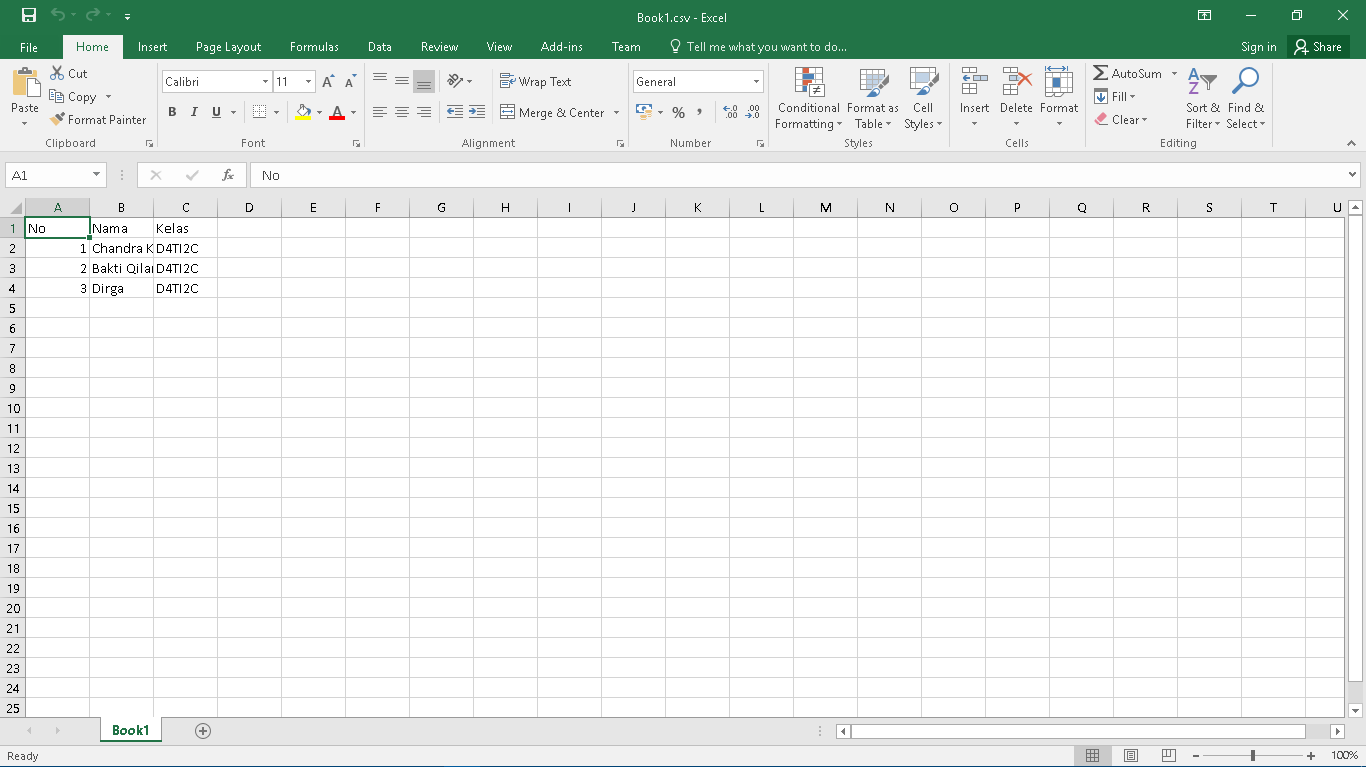
\includegraphics[width=10cm,height=10cm]{figures/4/1174079/Teori/contohmembuatcsvdengandata.png}
	\caption{Buat data CSV}
	\label{penanda}
	\end{figure}


 	\item Simpan dengan ektensi csv
	\begin{figure}[!htbp]
	\centering
	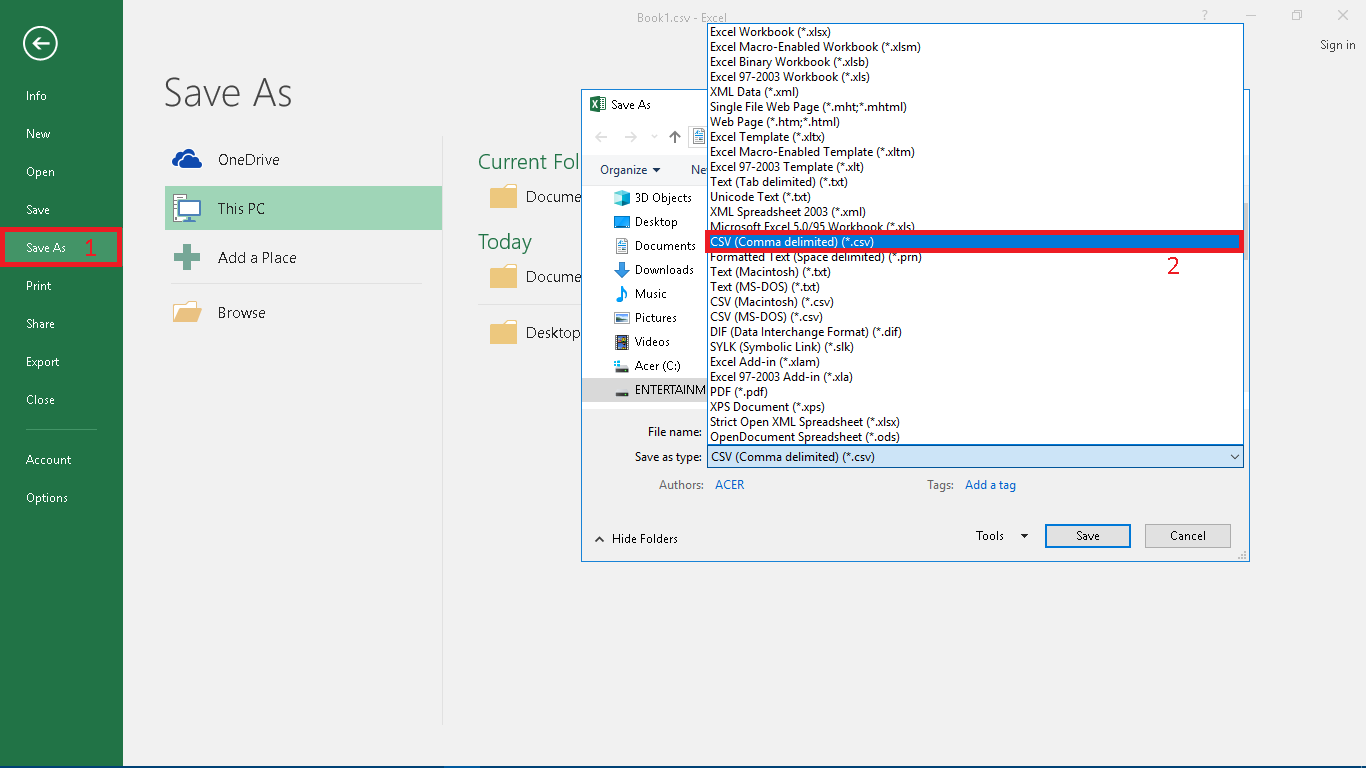
\includegraphics[width=10cm,height=10cm]{figures/4/1174079/Teori/menyimpanfiledenganformatcsv.png}
	\caption{Menyimpan CSV}
	\label{penanda}
	\end{figure}

	\item untuk membuka file csv, cari file yang anda simpan tadi
	\begin{figure}[!htbp]
	\centering
	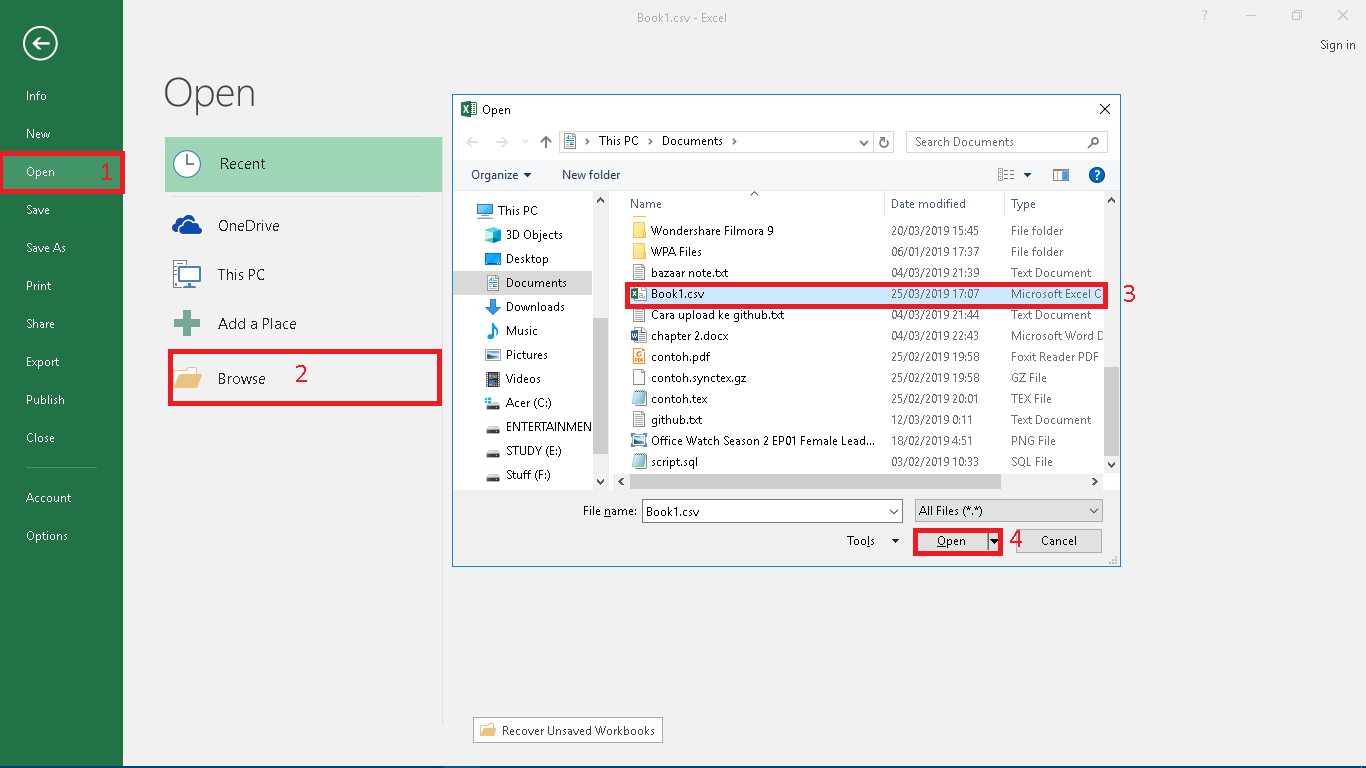
\includegraphics[width=10cm,height=10cm]{figures/4/1174079/Teori/bukafilecsv.png}
	\caption{Menyimpan CSV}
	\label{penanda}
	\end{figure}

\end{itemize}

\item Jelaskan sejarah library csv

CSV (Comma separated Values) adalah format data yang telah ada sebelum personal komputer hadir 10 tahun sebelumnya, CSV file pada tahun 1972 telah didukung oleh IBM Fortran, nama CSV sendiri mulai digunakan pada tahun 1983, menggunakan koma dan spasi sebagai pembatas, jadi karakter string yang tidak dikutip tidak bisa mengandung koma atau spasi, list CSV lebih mudah untuk diketik daripada data yang diatur berdasarkan kolum, dan lebih terhindar dari hasil yang salah jika di cetak pada media seperti punched card


\item Jelaskan sejarah library pandas

Pandas (Python Data Analysis Library) nama ini didapat dari istilah panel data dan juga istilah econometrik untuk data terstruktur multidimensi, Developer Wes McKinney mulai mengerjakan pandas pada tahun 2008, ketika saat AQR capital management sedang membutuhkan alat yang memiliki performa tinggi untuk melakukan analysis kuantitif tentang data finansial, sebelum keluar dari AQR, dia bisa membuat management percaya untuk supaya dia bisa membuat library open source. Chang She, bergabung pada tahun 2012 sebagai kontributor ke 2 untuk library pandas.


\item Jelaskan fungsi-fungsi yang terdapat di library csv
\begin{itemize}

	\item fungsi open di CSV
	
	Digunakan untuk membuka dan membaca file csv
	\lstinputlisting[firstline=10, lastline=20]{src/4/1174079/Teori/contohcsvchandra.py}

	\item fungsi write di csv
	
	Digunakan untuk menulis data ke file csv menggunakan writerow
	\lstinputlisting[firstline=7, lastline=12]{src/4/1174079/Teori/contohcsvwrite.py}
	
	\item fungsi write dengan parameter di csv
	
	Digunakan untuk menulis data ke file csv menggunakan writerow
	\lstinputlisting[firstline=7, lastline=14]{src/4/1174079/Teori/contohcsvwriteparameter.py}

\end{itemize}

\item Jelaskan fungsi-fungsi yang terdapat di library pandas
\begin{itemize}

	\item fungsi pandas read csv
	
	Digunakan untuk membuka, menganalisis, dan membaca file csv
	\lstinputlisting[firstline=7, lastline=9]{src/4/1174079/Teori/pandasreadchandra.py}
	
	\item fungsi pandas to csv
	Digunakan untuk menulis data ke file csv
	\lstinputlisting[firstline=7, lastline=13]{src/4/1174079/Teori/pandaswritechandra.py}

\end{itemize}

\end{enumerate}
